%%%%%%%%%%%%%%%%%%%%%%%%%%%%%%%%%%%%%%%%%%%%%%%%%%%
%
%  New template code for TAMU Theses and Dissertations starting Fall 2016.
%
%
%  Author: Sean Zachary Roberson 
%	 Version 3.16.09
%  Last updated 9/12/2016
%
%%%%%%%%%%%%%%%%%%%%%%%%%%%%%%%%%%%%%%%%%%%%%%%%%%%

%%%%%%%%%%%%%%%%%%%%%%%%%%%%%%%%%%%%%%%%%%%%%%%%%%%%%%%%%%%%%%%%%%%%%%
%%                           APPENDIX A 
%%%%%%%%%%%%%%%%%%%%%%%%%%%%%%%%%%%%%%%%%%%%%%%%%%%%%%%%%%%%%%%%%%%%%

\phantomsection

\chapter{\uppercase{Appendix}}\label{appendix1}

\begin{figure}[h]
\centering
  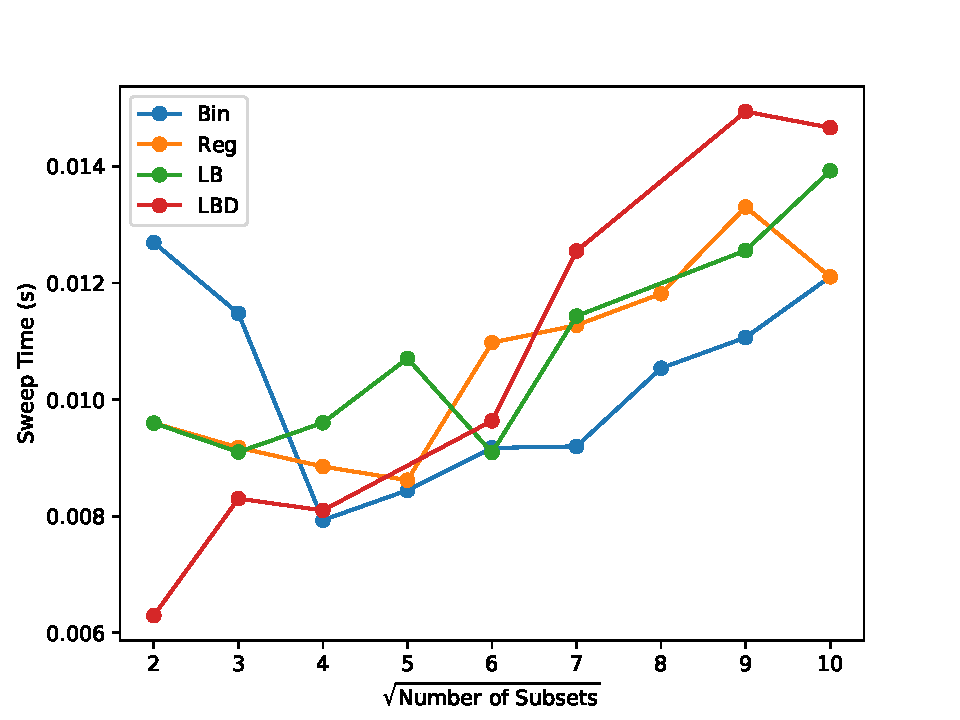
\includegraphics{../../figures/unbalanced_pins_opt_comparison.pdf}
  \caption{The time-to-solution for binary tree, regular, load-balanced and load-balanced-by-dimension cuts on the unbalanced pins mesh from 2 to 10 subsets in each dimension.}
\end{figure}
\begin{figure}[h]
\centering
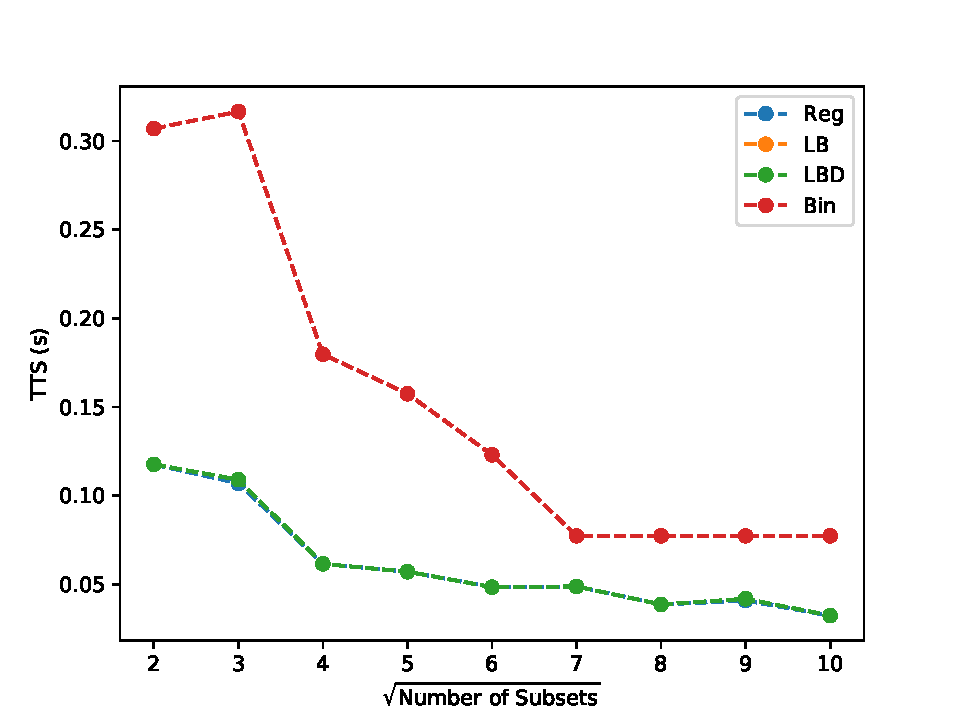
\includegraphics{../../figures/more_sparse_comp.pdf}
  \caption{The time-to-solution for binary tree, regular, load-balanced and load-balanced-by-dimension cuts on the ``heavier'' unbalanced pins mesh from 2 to 10 subsets in each dimension.}
\end{figure}
\begin{figure}[h]
\centering
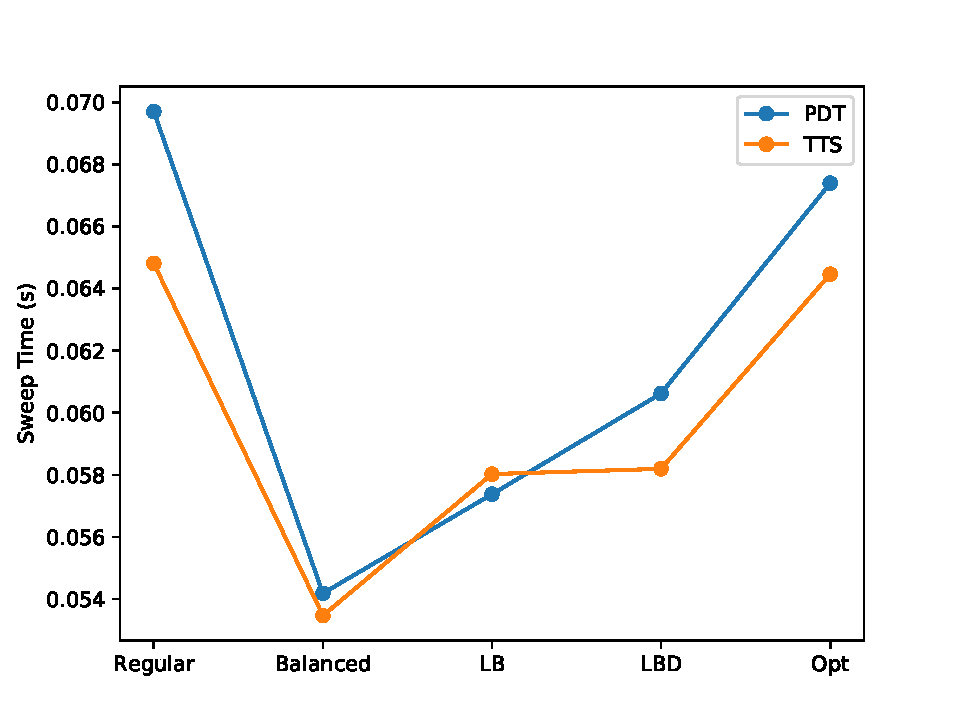
\includegraphics{../../figures/level2_sweep_comp.pdf}
\caption{The Level-2 mesh sweep times from the time-to-solution estimator for (1) regular cuts, (2) hand-balanced cuts, (3) load-balanced cuts, (4) load-balanced-by-dimension cuts, and (5) optimized cuts. }
\end{figure}
